%%%%%%%%%%%%%%%%%%%%%%%%%%%%%%%%%%%%%%%%%%%%%%%%%%%%%%%%%%%%%%%%%%%%%%%%%%%%%%%%
%
% \chapter{Installation}\label{chInstallation}
%
%%%%%%%%%%%%%%%%%%%%%%%%%%%%%%%%%%%%%%%%%%%%%%%%%%%%%%%%%%%%%%%%%%%%%%%%%%%%%%%%

This chapter is a step-by-step guide on how to install the graphical user interface GiD, the finite element computational tool ERMES 20.0 and the external solver library PETSc.

\section{Graphical user interface}

The recommended pre- and post- processor tool for ERMES 20.0 is GiD \cite{GiDWeb}. To install GiD, download the last version from \url{https://www.gidsimulation.com} and follow the instructions provided on that same webpage. After finishing the installation, open GiD, and click on the upper menu: \textbf{\underline{H}elp} $\rightarrow$ \textbf{Register GiD}, as shown in Figure \ref{GiD-RegisterMenu}:
\\
\begin{figure}[!h]
	\begin{center}
		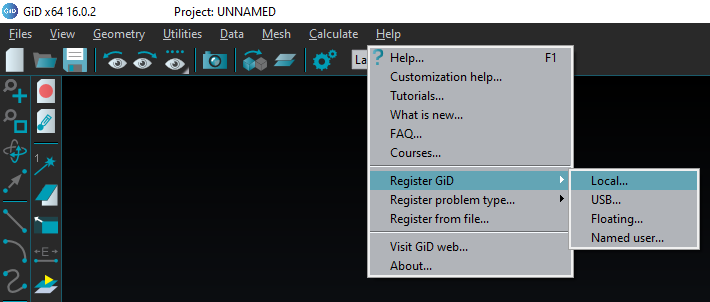
\includegraphics[width=0.95\textwidth]{Contents/Figures/GiD-RegisterMenu.png}
		\caption{Register GiD drop-down menu.}\label{GiD-RegisterMenu}
	\end{center}
\end{figure}
\\
Select \textbf{Local...} to register the local computer, \textbf{USB...} to register a USB stick attached to the local computer, \textbf{Floating...} to register a local network, or \textbf{Named user...} to attach the license to an email account. After clicking one of these options, a new window will appear with information related to the method selected and a link to obtain the password for a full professional license. Follow the link to get a one month free password or a permanent licence. The one month free license can be renewed up to three times for the same computer, USB stick, or email account. If the registration has been successful, the icon on the upper right corner of GiD will change colour as shown in Figure \ref{GiD-RegisterIcon}:
\\
\begin{figure}[!h]
\begin{center}

\includegraphics[width=0.5\textwidth]{Contents/Figures/GiD-RegisterButton.png}
\caption{GiD upper right icon indicating a successful registration.}\label{GiD-RegisterIcon}
\end{center}
\end{figure}

If a different pre- and post- processor software is preferred, the input files required by ERMES 20.0, and the output files it generates, can be edited and customized to meet the needs of any other pre- and post- processor tool (see Chapters \ref{chPreProcess} and \ref{chPostProcess} for a description of these input and output files).  

\section{ERMES 20.0}

If GiD is the chosen pre- and post- processor, the installation of ERMES 20.0 is very simple. The folder \path{\ERMES_20.0} is a problemtype of GiD. Therefore, the installation process consists in \textit{Copy\&Paste} the whole folder \path{\ERMES_20.0} inside the \path{\problemtypes} folder of GiD (located, for instance, in \path{C:\MySoftware\GiD 16.0.2\problemtypes}). The same installation process applies to Windows and Linux. 

To check that the installation has been done correctly, re-start GiD, and click on the GiD upper menu: \textbf{\underline{D}ata} $\rightarrow$ \textbf{Problem type}. ERMES 20.0 must appear in the drop-down menu as shown in Figure \ref{ERMES-Dopdrown}: 
\quad

\begin{figure}[H]
	\begin{center}
		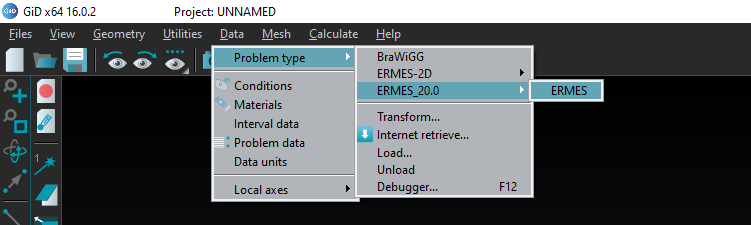
\includegraphics[width=\textwidth]{Contents/Figures/GiD-ERMES-Dropdown.png}
		\caption{GiD \textbf{\underline{D}ata} $\rightarrow$ \textbf{Problem type} drop-down menu showing ERMES 20.0 problemtype. Click on the ERMES submenu \textbf{\underline{D}ata} $\rightarrow$ \textbf{Problem type} $\rightarrow$ \textbf{ERMES\_20.0} $\rightarrow$ \textbf{ERMES} to start ERMES 20.0.}\label{ERMES-Dopdrown}
	\end{center}
\end{figure}

Click on the ERMES submenu \textbf{\underline{D}ata} $\rightarrow$ \textbf{Problem type} $\rightarrow$ \textbf{ERMES\_20.0} $\rightarrow$ \textbf{ERMES} and the ERMES logo, together with the ERMES menu bar, must appear as shown in Figure \ref{ERMES-Start}, indicating a successful installation of ERMES 20.0. If you open a GiD problem created previously with ERMES 20.0, you can convert it to the latest version (e.g., ERMES 20.0.4) by selecting ERMES 20.0.4 on the above submenu and choosing \textbf{Transform to new problem type}. The option \textbf{Reset to new problem type} must be selected only when the differences between versions are significant.
\quad\\
\quad\\[-0.75em]

\begin{figure}[H]
	\begin{center}
		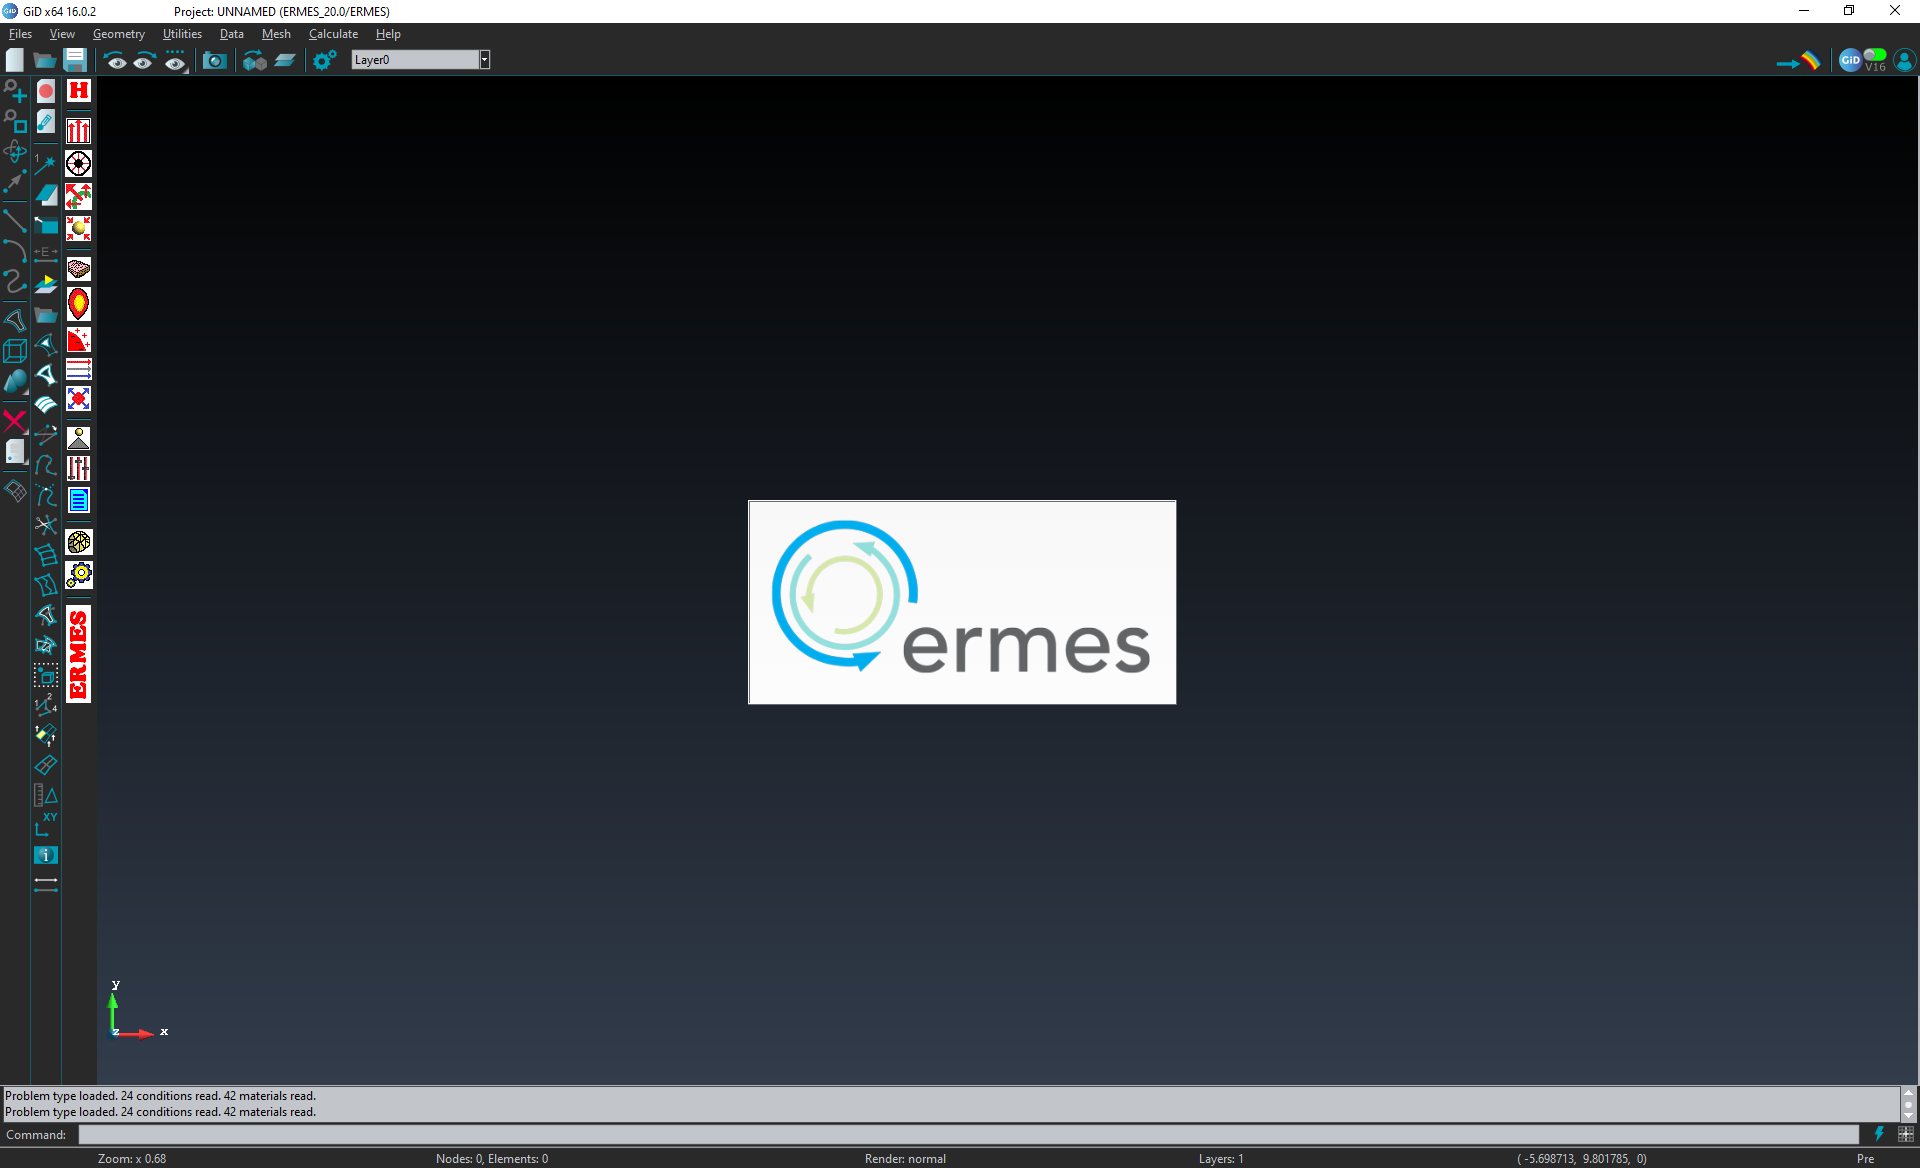
\includegraphics[width=0.96\textwidth]{Contents/Figures/ERMES-Start.png}
		\caption{ERMES 20.0 starting logo and menu bar.}\label{ERMES-Start}
	\end{center}
\end{figure}

If the ERMES 20.0 C++ source code needs to be recompiled (e.g. because it has been modified to add a new feature or because the local Linux distribution is not compatible with the distribution used to compile the executable provided in \path{\ERMES_20.0\ERMES.gid\execs\unix}), follow the instructions in \path{\ERMES_CPP_20.0\windows\README.txt} to compile ERMES for Windows, and the instructions in \path{\ERMES_CPP_20.0\unix\README.txt} to compile ERMES for Linux.

If the ERMES 20.0 C++ source code is recompiled, verify that the ERMES version called by the \path{ERMES.unix.bat} script for Linux or the \path{ERMES.win.bat} script for Windows matches the version you intend to use. These scripts, located in the GiD problem type folder \path{\ERMES_20.0\ERMES.gid}, are responsible for launching ERMES when the \textit{Calculate} button is clicked in GiD. They can also be modified to include additional program calls, delete files, or perform other custom tasks. For Linux systems, ensure that execution permissions are granted to the script \path{ERMES.unix.bat} and any executables it references. 

\section{PETSc solvers library}\label{ExternalSolversInstall}

Inside ERMES 20.0 there are implemented two iterative solvers (the bi-conjugate gradient and the transpose-free quasi-minimal residual) with diagonal preconditioning and OpenMP parallelization. These solvers are low-memory consuming and very efficient for well-conditioned matrices but, they can be insufficient for large, ill-conditioned linear systems. The recommended solver library for large complex linear systems is PETSc \cite{PETScWeb}, which offers access to direct and iterative solvers with several preconditioning options and MPI parallelization. PETSc can be installed in Windows and Linux. We recommend the installation in Linux and, if required in Windows, call PETSc from the Windows Subsystem for Linux 2 (WSL2). In the problemtype folder \path{\External_Solvers\PETSc} there is a bash file called \path{win2wsl.sh} that can be used as a template to call PETSc from Windows using WSL2. To install PETSc in Linux, follow these steps:
\begin{enumerate}\itemsep0em 
\item Download PETSc from its git repository to the local folder \path{/petsc}: 
   
\begin{small}\begin{lstlisting}
>> git clone -b release https://gitlab.com/petsc/petsc.git petsc
\end{lstlisting}\end{small} 
     
\item Configure PETSc using the command \path{./configure} inside the folder \path{/petsc} (check PETSc manual for configuration parameters definitions). Note that multiple configurations can be installed on the same machine, for instance:

\begin{small}\begin{lstlisting}
>> ./configure PETSC_ARCH=arch-complex-M1 --with-debugging=0 
   --download-mumps --download-scalapack --download-parmetis 
   --download-metis --download-ptscotch --with-64-bit-indices=1 
   --with-scalar-type=complex --download-mpich --download-cmake 
   --with-openmp --download-hwloc --with-cc=gcc --with-cxx=g++ 
   --with-fc=gfortran --download-fblaslapack --download-bison 
   --download-make
\end{lstlisting}\end{small}  	

\begin{small}\begin{lstlisting}
>> ./configure PETSC_ARCH=arch-complex-S1 --with-debugging=0 
   --download-superlu_dist --download-parmetis --download-metis 
   --download-ptscotch --with-64-bit-indices=1 
   --with-scalar-type=complex --download-mpich --download-cmake 
   --download-make --download-bison --with-cc=gcc --with-cxx=g++ 
   --with-fc=gfortran --download-fblaslapack 
\end{lstlisting}\end{small} 

\item Follow the instructions provided during the configuration process.
	
\item Add paths and preferred PETSC\_ARCH configuration to \path{.bashrc}:

\begin{small}\begin{lstlisting}
>> export PETSC_DIR=$HOME/petsc
>> export PETSC_ARCH=arch-complex-M1
>> export LD_LIBRARY_PATH=$LD_LIBRARY_PATH:
          $PETSC_DIR/$PETSC_ARCH/lib 
\end{lstlisting}\end{small}  

\item Reload \path{.bashrc} (or exit and log back in to your account):

\begin{small}\begin{lstlisting}
>> source $HOME/.bashrc
\end{lstlisting}\end{small}  	

\item Compile \path{PETScSolver.cpp} for the selected configuration by typing inside its folder location (e.g. \path{\External_Solvers\PETSc\Solver}):

\begin{small}\begin{lstlisting}
>> make PETScSolver
\end{lstlisting}\end{small}  

\item To run PETSc, use the Python scripts examples provided in the folder \path{\External_Solvers\PETSc}, or the batch files examples in \path{\Documents\Batch_Scripts}, or call PETSc directly from the command line using, for instance:

\begin{small}\begin{lstlisting}
>> mpiexec -n 6 ./PETScSolver -ksp_type bcgs -pc_type asm 
   -ksp_converged_reason -ksp_monitor_true_residual 
   -log_view -memory_view

>> mpiexec -n 8 ./PETScSolver -ksp_type richardson -pc_type lu 
   -pc_factor_mat_solver_type mumps -ksp_max_it 1 
   -log_view -ksp_error_if_not_converge

>> mpiexec -n 4 ./PETScSolver -ksp_type gmres -pc_type lu 
   -pc_factor_mat_solver_type mumps -ksp_max_it 1 
   -ksp_monitor_true_residual

>> mpiexec -n 8 ./PETScSolver -ksp_type richardson -pc_type lu 
   -pc_factor_mat_solver_type superlu_dist -ksp_max_it 1 
   -log_view -malloc_view
\end{lstlisting}\end{small}  	
\end{enumerate}
The above installation process can change depending on the Linux distribution. For further information, check the PETSc manual in \path{\External_Solvers\PETSc} or visit the webpage: \url{https://petsc.org}. 

If a different solver library is preferred (as, for instance, Python NumPy \cite{NumPyWeb}), check the Python scripts in \path{\External_Solvers\Python} and \path{\External_Solvers\PETSc} for examples of how to read the linear system produced by ERMES 20.0 and how to transform the matrix and vectors into different formats.
